% Copyright 2005-2016 Airbus-EDF-IMACS-Phimeca
% Permission is granted to copy, distribute and/or modify this document
% under the terms of the GNU Free Documentation License, Version 1.2
% or any later version published by the Free Software Foundation;
% with no Invariant Sections, no Front-Cover Texts, and no Back-Cover
% Texts.  A copy of the license is included in the section entitled "GNU
% Free Documentation License".
\renewcommand{\etapemethodo}{B}
\renewcommand{\nomfichier}{docref_B232_Spearman}
\renewcommand{\titrefiche}{Spearman correlation coefficient}

\Header

\MathematicalDescription{

  \underline{\textbf{Goal}} \vspace{2mm}

  This method deals with the parametric modelling of a probability distribution for a random vector $\vect{X} = \left( X^1,\ldots,X^{n_X} \right)$. It aims to measure a type of dependence (here a monotonous correlation) which may exist between two components $X^i$ and $X^j$.\vspace{2mm}

  \underline{\textbf{Principle}} \vspace{2mm}

  The Spearman's correlation coefficient $\rho^S_{U,V}$  aims to measure the strength of a monotonic relationship between two random variables $U$ and $V$. It is in fact equivalent to the Pearson's correlation coefficient after having transformed $U$ and $V$ to linearize any monotonic relationship (remember that Pearson's correlation coefficient may only be used to measure the strength of linear relationships, see \otref{docref_B231_Pearson}{Pearson's Correlation Coefficient}):
  \begin{align*}
    \rho^S_{U,V} = \rho_{F_U(U),F_V(V)}
  \end{align*}
  where $F_U$ and $F_V$ denote the cumulative distribution functions of $U$ and $V$.

  If we arrange a sample made up of $N$ pairs  $\left\{ (u_1,v_1),(u_2,v_2),\ldots,(u_N,v_N) \right\}$, the estimation of Spearman's correlation coefficient first of all requires a ranking to produce two samples $(u_1,\ldots,u_N)$ and $(v_1,\ldots,v_N)$. The ranking $u_{[i]}$ of the observation $u_i$ is defined as the position of $u_i$ in the sample reordered in ascending order: if $u_i$ is the smallest value in the sample $(u_1,\ldots,u_N)$, its ranking would equal 1; if $u_i$ is the second smallest value in the sample, its ranking would equal 2, and so forth. The ranking transformation is a procedure that takes the sample $(u_1,\ldots,u_N)$) as input data and produces the sample $(u_{[1]},\ldots,u_{[N]})$ as an output result.

  For example, let us consider the sample $(u_1,u_2,u_3,u_4) = (1.5,0.7,5.1,4.3)$. We therefore have $(u_{[1]},u_{[2]}u_{[3]},u_{[4]}) = (2,1,4,3)$. $u_1 = 1.5$ is in fact the second smallest value in the original, $u_2 = 0.7$ the smallest, etc.

  The estimation of Spearman's correlation coefficient is therefore equal to Pearson's coefficient estimated with the aid of the $N$ pairs $(u_{[1]},v_{[1]})$, $(u_{[2]},v_{[2]})$, \ldots, $(u_{[N]},v_{[N]})$:
  \begin{align*}
    \widehat{\rho}^S_{U,V} = \frac{ \displaystyle \sum_{i=1}^N \left( u_{[i]} - \overline{u}_{[]} \right) \left( v_{[i]} - \overline{v}_{[]} \right) }{ \sqrt{\displaystyle \sum_{i=1}^N \left( u_{[i]} - \overline{u}_{[]} \right)^2 \left( v_{[i]} - \overline{v}_{[]} \right)^2} }
  \end{align*}
  where $\overline{u}_{[]}$ and  $\overline{v}_{[]}$ represent the empirical means of the samples $(u_{[1]},\ldots,u_{[N]})$ and $(v_{[1]},\ldots,v_{[N]})$.

  The Spearman's correlation coefficient takes values between -1 and 1. The closer its absolute value is to 1, the stronger the indication is that a monotonic relationship exists between variables $U$ and $V$. The sign of Spearman's coefficient indicates if the two variables increase or decrease in the same direction (positive coefficient) or in opposite directions (negative coefficient). We note that a correlation coefficient equal to 0 does not necessarily imply the independence of variables $U$ and $V$. There are two possible situations in the event of a zero Spearman's correlation coefficient:
  \begin{itemize}
  \item the variables $U$ and $V$ are in fact independent,
  \item or a non-monotonic relationship exists between $U$ and $V$.
  \end{itemize}

  \begin{center}
    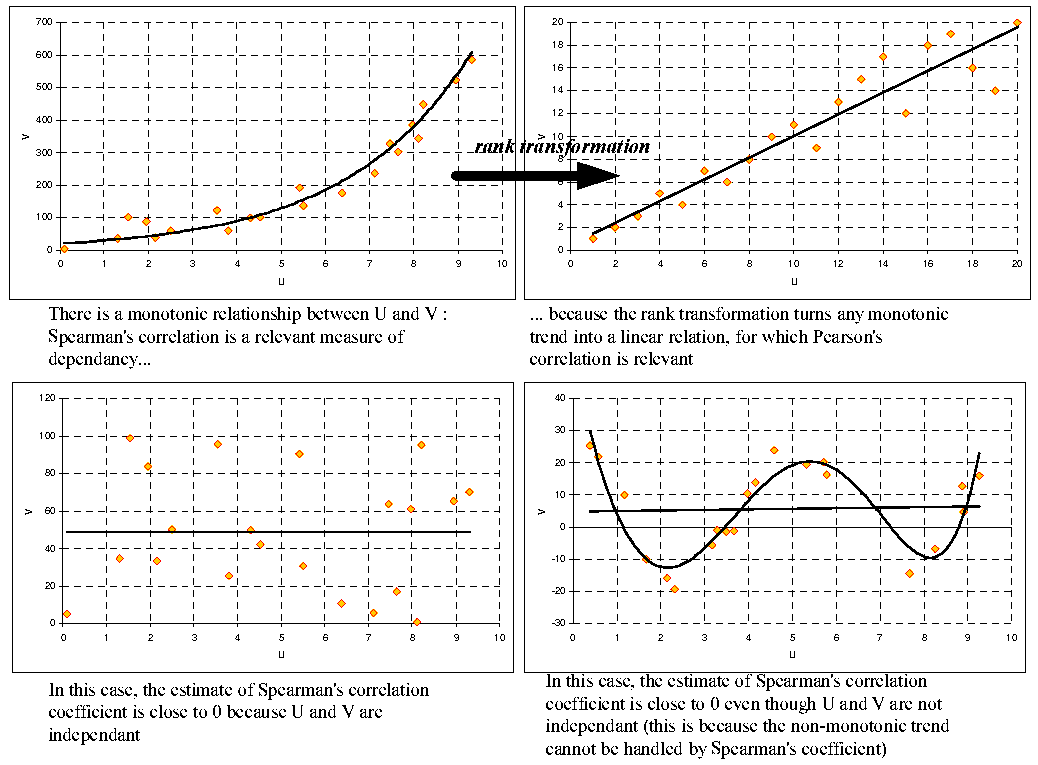
\includegraphics[width=0.5\textwidth]{Figures/spearman.pdf}
  \end{center}
}
{
  Spearman's coeeficient is often referred to as the rank correlation coefficient.
}



\Methodology{
  Spearman's correlation coefficient can be used in step B "Quantifying Sources of Uncertainty". Having defined the vector $\underline{X}$ of input variables in step A "Specifying Criteria and the Case Study", \otref{docref_B232_TestSpearman}{Spearman's Independence Test} shows how to test for the existence of a monotonous type of dependency between two components $X^i$ and $X^j$.
  Such a relationship should in fact be taken in to account so as not to falsify the results of step C "Propagation of Uncertainty".

  Spearman's correlation coefficient is also used in step C' "Sensitivity Analysis and Ranking of Sources of Uncertainty". If a propagation of uncertainty with Monte-Carlo simulation (step C, \otref{docref_C221_MonteCarloStd}{Mean and Variance Estimation using Standard Monte Carlo}) has been carried out, \otref{docref_Cprime212_Spearman}{Spearman's Ranking} shows the user how to class the components of the input vector $\underline{X}$ according to their impact on the uncertainty of a final variable / output variable defined in step A.
}
{
  Regardless of the method used in step B or step C', we recall that the Spearman's coefficient is only useful in measuring a monotonous relationship between two variables. Readers are referred to the following references:
  \begin{itemize}
  \item Saporta, G. (1990). "Probabilités, Analyse de données et Statistique", Technip
  \item Dixon, W.J. \& Massey, F.J. (1983) "Introduction to statistical analysis (4th ed.)", McGraw-Hill
    % \item NIST/SEMATECH e-Handbook of Statistical Methods, http://www.itl.nist.gov/div898/handbook/
    % \item D'Agostino, R.B. and Stephens, M.A. (1986). "Goodness-of-Fit Techniques", Marcel Dekker, Inc., New York.
  \item Bhattacharyya, G.K., and R.A. Johnson, (1997). "Statistical Concepts and Methods", John Wiley and Sons, New York.
  \item Sprent, P., and Smeeton, N.C. (2001). "Applied Nonparametric Statistical Methods -- Third edition", Chapman \& Hall
    % \item Burnham, K.P., and Anderson, D.R (2002). "Model Selection and Multimodel Inference: A Practical Information Theoretic Approach", Springer
\end{itemize}}
